\chapter{Introducción a los chatbots}
\label{cha:IntroChatbot}

En este capítulo se tratará de abordar uno de los conceptos fundamentales en los que se basa el trabajo realizado, los chatbots. En el Apartado \ref{sec:DefinicionChatbot} se describe qué es un chatbot y en qué contextos se utiliza. En el Apartado \ref{sec:PlataformasChatbot} se explicará las actuales plataformas para el desarrollo de chatbots, sus características y la solución que se ha adoptado en este trabajo.

\section{Definición y contexto de uso}
\label{sec:DefinicionChatbot}

Un chatbot se puede describir como un software para automatizar infinidad de tareas que actualmente desarrollan los usuarios por si mismos, como reservar un restaurante para cenar, añadir un evento al calendario u obtener información \cite{Wagner2016}.

Un concepto que habitualmente se confunde o se solapa (en cierta medida) con los chatbots son los asistentes personales o asistentes digitales. Ambas ideas comparten algunas características que se presentan a continuación:
\begin{itemize}
	\item Tanto los chatbots como los asistentes personales disponen (o pueden disponer) de interfaz textual o por voz.
	\item Ambas ideas tienen como objetivo automatizar tareas cotidianas.
	\item Son capaces de integrar múltiples servicios.
\end{itemize}

Sin embargo, presentan una diferencia principal. Un chatbot está orientado a resolver ciertos problemas, digamos que es experto en un ámbito concreto, puede actuar como representante de una empresa o un servicio. Mientras tanto un asistente personal juega el papel de oráculo y tiene que lidiar con cualquier tipo de tarea \cite{Wright2016}.

Lo que las definiciones dejan claro es que un bot conversacional tiene un propósito especifico y que en lineas generales es un software que debe de lidiar con o resolver tareas cotidianas del usuario.

A continuación se puede ver un ejemplo. En la Figura \ref{fig:Politibot} se puede observar la interacción que tiene un usuario con un chatbot llamado Politibot. Politibot\footnote{Sitio web de @politibot: \url{https://politibot.es/}} es un agente conversacional que permite ofrecer información acerca de las elecciones generales de España. En la imagen izquierda Figura \ref{fig:Politibot} se puede ver cómo el bot recaba cierta información del usuario (rango de edad, localización) para de esta manera ofrecer información más relevante para el elector. En la imagen derecha, el usuario pregunta por los resultados de las elecciones, a lo que el chatbot proporciona una respuesta personalizada, mostrando los datos de las elecciones generales, pero también los de su provincia.

Detrás de un chatbot de estas características se aúnan diferentes servicios: bases de datos con las preferencias de los usuarios, sistemas de localización o datos extraídos de servicios web para las noticias o los resultados.

\begin{figure}[htb]
	\centering
	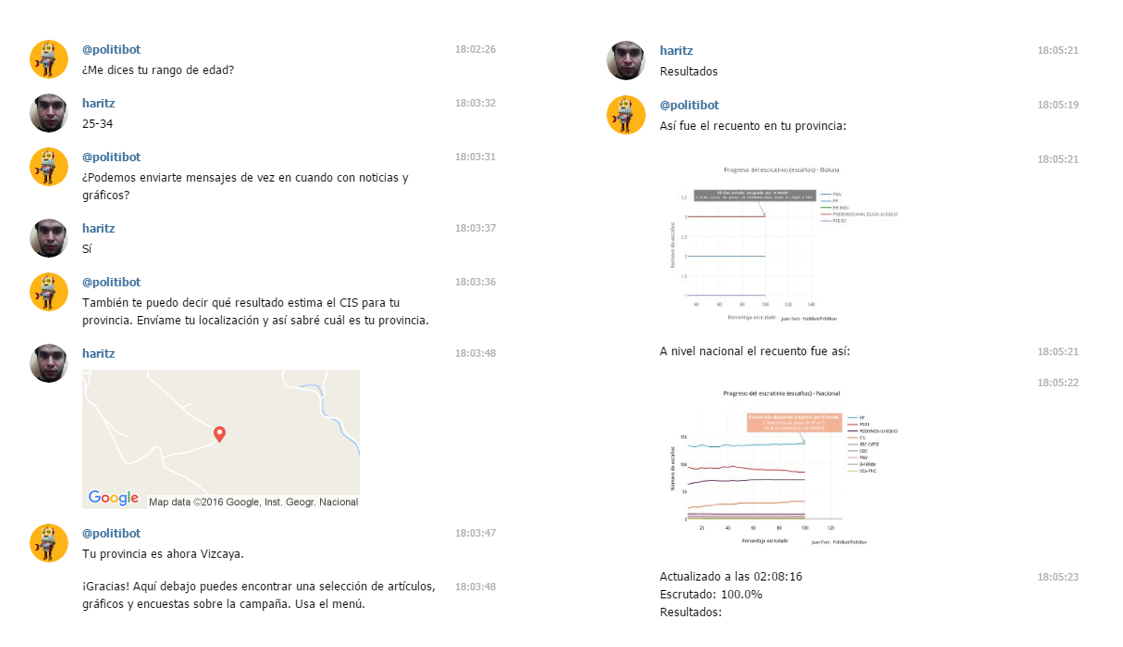
\includegraphics[width=0.8\textwidth]{./figs/Politibot.png}
	\caption{Un chatbot que informa sobre las elecciones españolas del 26-J ofreciendo información personalizada a cada usuario.}
	\label{fig:Politibot}
\end{figure}

Cualquiera puede pensar que los bots son un concepto nuevo dentro de las tecnologías de información. Sin embargo, es una idea que lleva desde los comienzos de la informática (uno de los pioneros fue el proyecto ELIZA\footnote{Proyecto ELIZA, un chatbot que simulaba a una psicóloga: \url{https://en.wikipedia.org/wiki/ELIZA}}), aunque en los últimos años está en crecimiento \cite{Ferrara2016}. Esto es debido al aumento de las redes sociales y de los dispositivos interconectados dentro de lo que se conoce cómo el Internet de las Cosas \footnote{Utilización de chatbots como interfaces para el Internet de las cosas: \url{https://iot.telefonica.com/blog/using-smart-chatbots-as-an-iot-interface}}.

Los chatbots proporcionan una interfaz de comunicación en la que se reduce el coste frente a la interacción humana \cite{Dans2016}. De igual manera también porque esta interacción ejerce menor presión en el usuario que quiere realizar consultas. Un bot está disponible para atender consultas 24 horas al día los 7 días de la semana, y puede atender simultáneamente consultas de múltiples usuarios, a diferencia de los humanos.

En el próximo Apartado \ref{sec:PlataformasChatbot} se hará hincapié en las plataformas que ofrecen los chatbots y las características de los mismos.

\section{Plataformas para desarrollo de agentes conversacionales}
\label{sec:PlataformasChatbot}

Como se ha mencionado en el apartado anterior, los chatbot existen desde hace varias décadas. Sin embargo, con el uso de las tecnologías móviles y el aumento del uso de aplicaciones de chat para conversar \cite{Montag2015}, ha hecho que los bots se hayan puesto en boga nuevamente.

Hay que diferenciar dos aspectos a la hora de hablar de plataformas para los chatbots. Por un lado existen las plataformas donde tiene el chatbot su interfaz, es decir, en qué aplicación o servicio mediante el cual chatea el usuario con el bot, que será en la que se centra este apartado. Por otro lado está la plataforma de desarrollo de los bots, que es la librería o servicio que se utiliza para desarrollar un chatbot que después será desplegado en una o más plataformas.

En referencia a la interfaz de los chatbots, en la actualidad muchas empresas ofrecen su plataforma como interfaz para interactuar con los chatbots. Entre ellas destacan: Facebook, Twitter, Telegram, Microsoft Skype o Slack. Sin embargo, empresas como Kik llevan trabajando años en el area de los chatbots \footnote{¿Como predijo Kik el crecimiento del uso de los chatbots? \url{https://backchannel.com/how-kik-predicted-the-rise-of-chat-bots-2eaf9027b86e}}.

La plataforma de desarrollo están muy ligada a la interfaz. Volviendo al ejemplo de politibot, en la Figura \ref{fig:PolitibotBotones} se observa como la interfaz de Telegram proporciona botones con las diferentes opciones que el usuario puede elegir para interactuar con el bot. Esta característica es particular de Telegram, que por ejemplo Slack no dispone. Sin embargo, otras plataformas ofrecen otras características que Telegram no contempla.
\begin{figure}[htb]
	\centering
	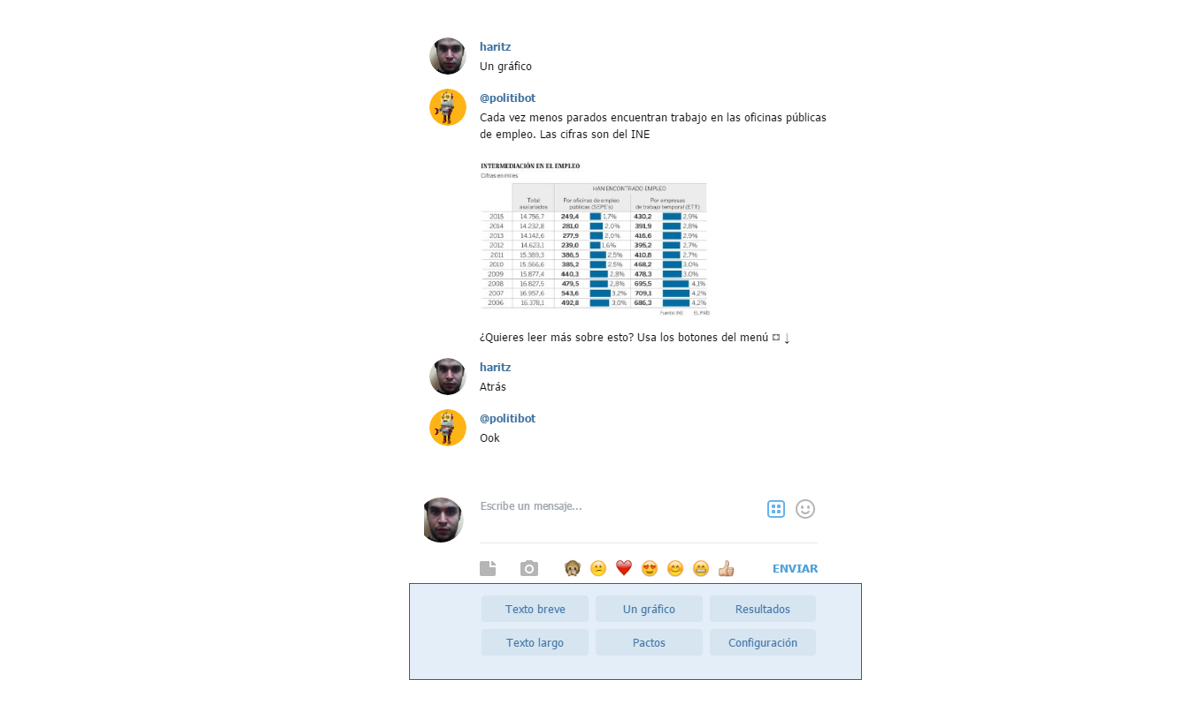
\includegraphics[width=0.8\textwidth]{./figs/PolitibotBotones.png}
	\caption{El chatbot define las posibles opciones que ofrece para responder mediante botones en lugar de esperar un mensaje textual.}
	\label{fig:PolitibotBotones}
\end{figure}

Es por ello que existen muchas plataformas de desarrollo. Algunas de ellas, como Microsoft Bot Framework \footnote{Microsoft Bot Framework: \url{https://dev.botframework.com/}} ofrecen soporte multiplataforma (Telegram, Slack, Skype, Messenger,...), otras como la API de Telegram\footnote{Telegram bot API: \url{https://core.telegram.org/bots}} es exclusiva para Telegram.

En este trabajo, se ha decidido trabajar con la librería Botkit \footnote{Sitio web de Botkit: \url{https://github.com/howdyai/botkit}}. Las principales razones son las siguientes:
\begin{itemize}
	\item Es multiplataforma, actualmente soporta Slack, Facebook Messenger\footnote{Sitio web de Facebook Messenger:\url{https://facebook.com/}} y Twilio IP Messaging\footnote{Sitio web de Twilio: \url{https://www.twilio.com/docs/api/ip-messaging}}.
	\item Es software libre, lo que permite ver el código fuente y modificarlo, además de que no tiene ningún coste económico.
	\item Es sencillo de desarrollar, permite abstraer bastante la implementación a bajo nivel de los chatbots, que es compleja debido a las llamadas asíncronas y las conexiones a múltiples servicios que trabaja por debajo.
\end{itemize}

Para profundizar en las características de implementación sobre Botkit es conveniente revisar el Capítulo \ref{cha:Implementation}.